
\subsection{Change of Variables and the Jacobian}
\begin{example}{Annoying Example}
Lets consider the volume beneath the surface $f(x,y)=1$ where $D$ is the disk of radius 1. Clearly this is just a cylinder with radius 1 and height 1, and our volume should simply be $\pi$. But for the sake of example, lets set this up as a double integral.
$$\iint_D 1 \ dA=\int_{-1}^{1}\int_{-\sqrt{1-x^2}}^{\sqrt{1-x^2}}1\ dy\ dx. $$
Evaluating the inner integral leads us quickly to:
$$\int_{-1}^{1}2\sqrt{1-x^2}\ dx $$ which you may recall from Calculus II as a tedious trig sub where $x=\sin\theta$. There has to be an easier way!
\end{example}

In fact, there is an easier way, related to a method of integration you've been using for almost as long as you've been integrating! Remember the method of $u$-substitution, where you evaluate a tricky single integral by substituting some $u$ for $x$. Of course, you have to be careful-- and there's a trade off. When doing your $u$ substitution, you must not only replace $x$ with $u$, but also replace $dx$ with $du$. We use an expansion of this technique to do substitutions, or changes of variables for multiple integrals.

Why are these changes of variables useful? Well, often times an annoying object in one set of variables is a much less annoying object in another set of variables.

\begin{example}{An Ellipse No More}
Consider the ellipse $x^2+\frac{y^2}{36}=1.$ If we use the change of variables $x=\frac{u}{2}$ and $y=3v$, then we substitute:
\begin{align*}
x^2+\frac{y^2}{36}=&1\\
\left(\frac{u}{2}\right)^2+\frac{(3v)^2}{36}=&1\\
\frac{u^2}{4}+\frac{v^2}{4}=&1\\
u^2+v^2=4.
\end{align*}
This is a circle with radius 2.
\end{example}

\begin{exercise}{A Transformation}
Consider the region that is the triangle with vertices at $(0,0)$, $(1,2)$ and $(2,1)$. This is the region bounded by the lines \begin{align*}
y=&2x\\
y=&\frac{1}{2}x\\
y=&3-x.
\end{align*}
Use the transformation $x(u,v)=u+v$ and $y(u,v)=u-v$ to transform the region, then give the bounds for the region in terms of your new variables, $u$ and $v$.
\end{exercise}

However, note that a change of variables for integration comes with a cost. In $u$-substitution, that cost was replacing $dx$ with a $du$ term. We'll expand this idea using the \textbf{Jacobian}.

\begin{example}{Why Do We Need the Jacobian?}
It should be relatively clear that when we change our variables to describe a region more simply, we end up changing the area of the region. For example, lets consider the region $R$ bounded by $x^2+y^2=9$, $x=0$ and $y=0$. This is a quarter disc with radius 3.

\vspace{1em}
\begin{center}
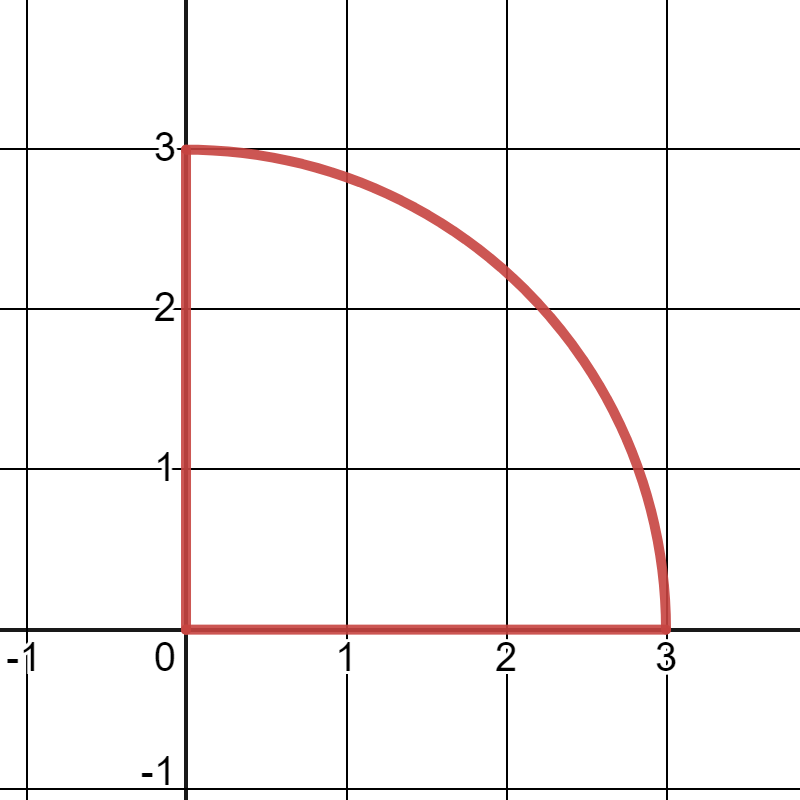
\includegraphics[scale=0.2]{Figures/521}\\Quarter Disc of Radius 3.
\end{center}
\vspace{1em}

Imagine that we want to integrate $f(x,y)=1+x+2y$ over $R$. That is, we want to find $$\iint_R 1+x+2y\ dA. $$ This is certainly possible, but quite annoying. So instead, we might think that while describing a circle in rectangular coordinates is tedious, this region is incredibly simple to describe in polar coordinates! That is, if we were to use the change of variables $x=r\cos\theta$ and $y=r\sin\theta$, then we get that our region is just 
$$R=\left\{(r,\theta): \ 0\leq\theta\leq \frac{\pi}{2},\ 0\leq r\leq 3 \right\}$$ 
and our function changes to 
$$f_t(r,\theta)=1+r\cos\theta+2r\sin\theta.$$ 
The double integral itself has no idea what polar coordinates are. So integrating 
$$\int_{0}^{3}\int_{0}^{\pi/2}1+r\cos\theta+2r\sin\theta\ d\theta \ dr $$ 
is just a double integral over a rectangular region, complete with being able to commute our integrals! In fact, that rectangular region just looks like this!

\vspace{1em}
\begin{center}
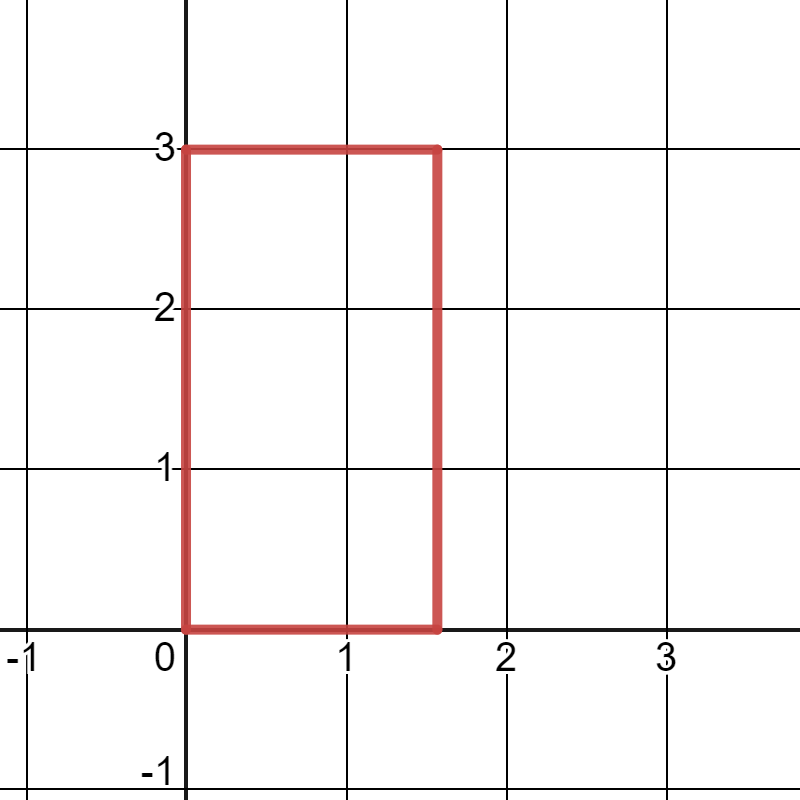
\includegraphics[scale=0.2]{Figures/522}\\$R$ in ``Polar'' Coordinates.
\end{center}
\vspace{1em}

Note also that our new surface, $$f_t(r,\theta)=1+r\cos\theta+2r\sin\theta\ $$ is much harder to describe, but still has the correct height above corresponding sections of $R$. That is, we can take any $(x,y)$ point in $R$ like $(\sqrt{2},\sqrt{2})$, then plug that into $f(x,y)$ to get 
$$f(\sqrt{2},\sqrt{2})=1+\sqrt{2}+2\sqrt{2}=1+3\sqrt{2}. $$ 
Then, we take that same point point, convert it to polar coordinates, 
$$(\sqrt{2},\sqrt{2})\to\left(2,\frac{\pi}{4}\right) $$ 
and when we plug that into $f_t(r,\theta)$, we get the same result, 

\begin{align*}
f_t\left(2,\frac{\pi}{4}\right)=&1+2\cos\left(\frac{\pi}{4}\right)+2\left(2\sin\left(\frac{\pi}{4}\right)\right)\\
=&1+2\left(\frac{\sqrt{2}}{2}\right)+4\left(\frac{\sqrt{2}}{2}\right)\\
=&1+\sqrt{2}+2\sqrt{2}\\
=&1+3\sqrt{2}.
\end{align*}

However, when we integrate, we get two different results:

\begin{align*}
\int_{0}^{3}\int_{0}^{\sqrt{1-x^2}} 1+x+2y\ dy\ dx=&27+\frac{9\pi}{4}\approx34.069\\
\int_{0}^{3}\int_{0}^{\pi/2}1+r\cos\theta+2r\sin\theta\ d\theta \ dr=&\frac{27}{2}+\frac{3\pi}{2}\approx18.212.
\end{align*}

This makes sense! After all, these regions have two different areas. Our original $R$ has an area of $\frac{9\pi}{4} $ and the polar version has an area of $\frac{3\pi}{2}$, so the original version is $1.5$ times larger than the polar version. But just multiplying by $1.5$ doesn't fix the problem, so what's going on here?

\vspace{1em}

The problem is that when we convert to polar coordinates, while we are scaling the region, we are not scaling every part of the region at the same rate. For example, consider the two subregions of $R$ below.

\vspace{1em}
\begin{center}
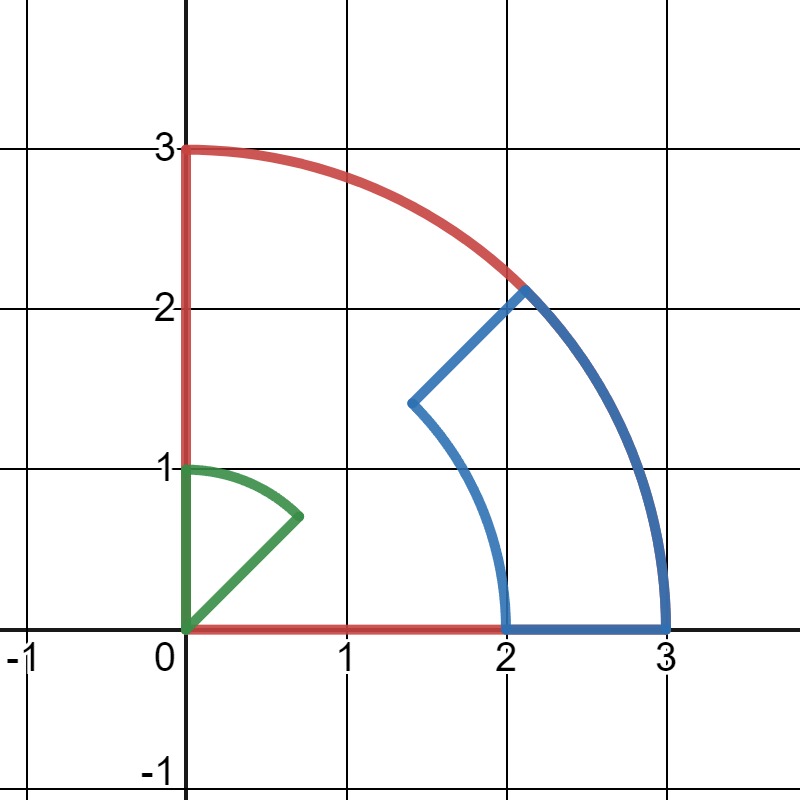
\includegraphics[scale=0.2]{Figures/523}\qquad 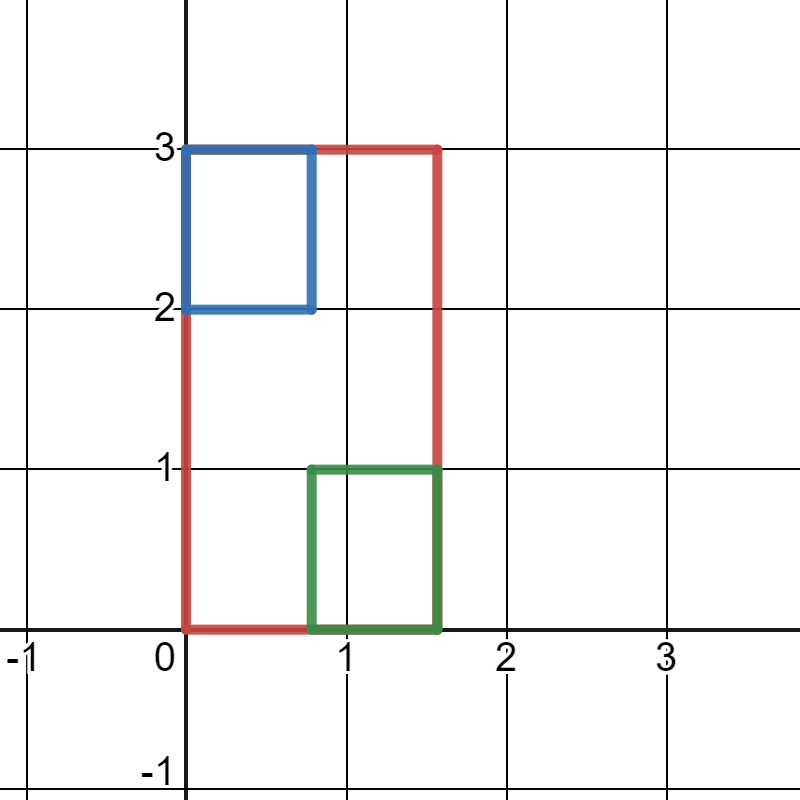
\includegraphics[scale=0.2]{Figures/524}\\Sub-regions of $R$ in Rectangular and Polar Coordinates.
\end{center}
\vspace{1em}

In both of the above graphs, the blue sub-region can be described by the polar coordinates 
$$R_b=\left\{(r,\theta): \ 0\leq\theta\leq \frac{\pi}{4},\ 2\leq r\leq 3 \right\}$$ 
and the green sub-region can be described by the polar coordinates
$$R_g=\left\{(r,\theta): \ \frac{\pi}{4}\leq\theta\leq \frac{\pi}{2},\ 0\leq r\leq 1 \right\}$$ 
In the left image, which is before the polar transformation, the blue sub-region is clearly \textit{larger} than the green one, while in the right image, after the polar transformation, the two regions are the same exact size! This transformation is scaling different parts of this region by different amounts. So we need some way of re-scaling the region after the transformation to ensure that our integrals match up. That scaling factor depends on the \textbf{Jacobian.}
\end{example}

So what is this magical Jacobian? Well, it's a matrix, so that's fun. In Linear Algebra, we write transformations between two different coordinate systems (or vector spaces) as matrix multiplication. Well, we specifically refer to \textit{linear} transformations as matrix multiplication, and of course, our problem is that often times the transformations we want to use here are often \textit{not} linear. The Jacobian is the matrix that gives a linear approximation of our non-linear transformations. Of course, how do we do linear approximations? You guessed it, lots of derivatives! The Jacobian essentially collects all the partial derivatives of each function in our transformation and stores them in a matrix.

\begin{definition}{Jacobian}
Let $\vcf$ be a function $\vcf: \bbr^n\to\bbr^n$. That is, $\vcf$ is a transformation between 2 $n$-dimensional vector spaces, or $$\vcf=\bmat{f_1(x_1,x_2,\ldots,x_n)\\ f_2(x_1,x_2,\ldots,x_n)\\ \vdots \\  f_n(x_1,x_2,\ldots,x_n)}. $$ Then the \textbf{Jacobian} of $\vcf$ is the matrix
$$J=\bmat{\frac{\del \vcf}{\del x_1} & \frac{\del \vcf}{\del x_2} & \cdots & \frac{\del \vcf}{\del x_n}}=\bmat{(\nabla f_1)^T\\(\nabla f_2)^T\\ \vdots\\ (\nabla f_n)^T}=
\bmat{
\frac{\del f_1}{\del x_1} & \cdots & \frac{\del f_1}{\del x_n} \\
\vdots  & \ddots & \vdots \\
\frac{\del f_n}{\del x_1} & \cdots & \frac{\del f_n}{\del x_n}
}$$ where $(\nabla f_i)^T$ is the transpose (to a row vector) of the gradient of $f_i$.

\vspace{1em}

In particular, for a $2$-dimensional change of coordinates, $x=x(u,v)$ and $y=y(u,v)$, the Jacobian is $$J=\bmat{\frac{\del x}{\del u} & \frac{\del x}{\del v} \\ \frac{\del y}{\del u} & \frac{\del y}{\del v}}=\bmat{x_u & x_v \\ y_u & y_v}.$$ For a $3$-dimensional change of coordinates, $x=x(u,v,w)$, $y=y(u,v,w)$ and $z=z(u,v,w)$, then the Jacobian is $$J=
\bmat{
\frac{\del x}{\del u} & \frac{\del x}{\del v} & \frac{\del x}{\del w}\\
\frac{\del y}{\del u} & \frac{\del y}{\del u} & \frac{\del y}{\del w}\\
\frac{\del z}{\del u} & \frac{\del z}{\del v} & \frac{\del z}{\del w}
}=\bmat{x_u & x_v & x_w \\ y_u & y_v & y_w \\ z_u & z_v & z_w}.$$
\end{definition}

What we really want, actually, to complete our transformations and to be able to integrate according to our new variables, is the \textbf{determinant} of the Jacobian. \hyperlink{det}{We first did determinants way back when we covered the cross product.} So how do these pieces come together? Well, the determinant of the Jacobian, $\det(J)$, tells us what non-linear scaling factor we need to apply to make our integrals before and after the transformation the same!

\begin{claim}{Change of Variables, Double Integral}
Consider the surface $f(x,y)$ over the region $R$. When applying the transformation $x=x(u,v)$, $y=y(u,v)$, the region becomes $S$, the function transforms to $f_t(u,v)$ and $$\iint_R f(x,y)\ dA=\iint_S f_t(u,v)\cdot |\det(J)|\ d\ca{A} $$ where $d\ca{A}$ indicates that the variables of integration are now $u$ and $v$ instead of $x$ and $y$ and $|\det(J)|$ is the absolute value of the determinant of the Jacobian of the transformation.
\end{claim}

\begin{claim}{Change of Variables, Triple Integral}
Consider the function $f(x,y,z)$ over the region $R$. When applying the transformation $x=x(u,v,w),$ $y=y(u,v,w)$ and $z=z(u,v,w)$, the region becomes $S$, the function transforms to $f_t(u,v,w)$ and $$\iiint_R f(x,y,z)\ dV=\iiint_S f_t(u,v,w)\cdot |\det(J)| \ d\ca{V} $$ where $d\ca(V)$ indicates that the variables of integration are now $u$, $v$ and $w$ instead of $x$, $y$ and $z$ and $|\det(J)|$ is the absolute value of the determinant of the Jacobian of the transformation.
\end{claim}

Lets use this to compute the Jacobians and their determinants in general for transformations for double and triple integrals!

\begin{exercise}{Jacobian Determinants}
\begin{enumerate}
\item Consider the transformation $x=x(u,v)$ and $y=y(u,v)$. Compute $\det(J)$, the determinant of the Jacobian of a 2-dimensional transformation. 
\vspace{1em}
\item Consider the transformation $x=x(u,v,w)$, $y=y(u,v,w)$ and $z=z(u,v,w)$. Compute $\det(J)$, the determinant of the Jacobian of a 3-dimensional transformation.
\end{enumerate}
\end{exercise}

\begin{exercise}{The Transformation from Before!}
Consider the region $R$ that is the triangle with vertices at $(0,0)$, $(1,2)$ and $(2,1)$. This is the region bounded by the lines. You used the transformation $x(u,v)=u+v$ and $y(u,v)=u-v$ to transform this region before. Now find the Jacobian and $|\det(J)|$ for this transformation. Then use this transformation to evaluate the integral: $$\iint_R 2xy \ dA.$$ 
\end{exercise}

Now we can refer back to our example!

\begin{example}{A Less Annoying Example}
Lets return to the beginning-- the volume beneath the surface $f(x,y)=1$ where $D$ is the disk of radius 1. But lets convert to polar coordinates. That is, convert from variables $(x,y)$ to variables $(r,\theta)$. Then $x=x(r,\theta)=r\cos\theta$ and $y=y(r,\theta)=r\sin\theta$. We need to do a few tasks:
\vspace{1em}
\begin{itemize}
\item Convert our bounds: The disk of radius 1 in polar coordinates is $$S=\big\{(r,\theta):\ 0\leq r\leq 1,\ 0\leq\theta\leq 2\pi \big\}.$$
\vspace{1em}
\item Convert our function: Since $f(x,y)=1$, $f_t(r,\theta)=1$ also.
\vspace{1em}
\item Compute our Jacobian and its determinant: 
\begin{align*}J=&\bmat{x_r & x_\theta\\y_r&y_\theta} \\
=&\bmat{\frac{\del}{\del r}(r\cos\theta)& \frac{\del}{\del \theta}(r\cos\theta)\\ \frac{\del}{\del r}(r\sin\theta)& \frac{\del}{\del \theta}(r\sin\theta)}\\
=&\bmat{\cos\theta & -r\sin\theta\\ \sin\theta & r\cos\theta}.
\end{align*}
Then the determinant:
\begin{align*}
\det(J)=&\vmat{\cos\theta & -r\sin\theta\\ \sin\theta & r\cos\theta}\\
=& (\cos\theta)(r\cos\theta)-(-r\sin\theta)(\sin\theta)\\
=& r\cos^2\theta+r\sin^2\theta\\
=&r(\cos^2\theta+\sin^2\theta)\\
=&r.
\end{align*}
\end{itemize}
Then we can rewrite our integral:
$$\iint_D 1 \ dA=\iint_S 1 |r| \ d\ca{A}=\int_{0}^{2\pi}\int_{0}^1 r \ dr \ d\theta.$$
Then we need only evaluate the iterated integral.

\begin{align*}
\int_{0}^{2\pi}\int_{0}^1 r \ dr \ d\theta=& \int_{0}^{2\pi}\Bigg[\frac{r^2}{2} \Bigg]_{r=0}^{r=1} \ d\theta\\
=&\int_0^{2\pi}\frac{1}{2} \ d\theta \\
=&\Bigg[\frac{\theta}{2} \Bigg]_{\theta=0}^{\theta=2\pi} \\
=&\pi.
\end{align*}

\end{example}

\begin{exercise}{Changing Coordinates}
Let $R$ be the diamond shaped region with vertices at $(0,0)$, $(5/2,5/2)$, $(5,0)$ and $(5/2,-5/2)$. Evaluate the integral using the transformation $x(u,v)=2u+3v$, $y(u,v)=2u-3v$. $$\iint_R x+y \ dA .$$ 
Hint: Draw a graph of the region before the transformation. What are the equations of the lines that bound the diamond shape? What happens to the equations of those lines when you apply the desired transformation?
\end{exercise}

\begin{exercise}{U-Substitution and the Jacobian}
Consider the integral $$\int_{0}^1 x\sqrt{1+x^2} \ dx.$$
Traditionally, we would solve this integral using the $u$-substitution, $u=1+x^2$. Instead, consider the change of variables $x(u)=\sqrt{u-1}$, and compute the integral using our change of variables formula. Note that if our Jacobian is a $1\times 1$ matrix, like $$J=\bmat{j_1}, $$ then $\det(J)=j_1$.
\end{exercise}